\subsection{Assignment}
The assignment was \textbf{Extend the processor from the previous assignment by changing the 
data path to a pipeline}, the including tasks were to

\begin{itemize}
  \item Add pipeline registers to all the stages described in Figure \ref{pipeline-registers}.
  \item Optimize performance by adding data-forwarding techniques to the pipeline.
  \item Optimize performance by adding hazard-detection techniques
\end{itemize}
The assignment also specified that at least the following instructions from 
the MIPS Architecture should be implemented

\begin{description}
  \item[ALU] \hfill \\
    ADD - Addition \\
    SUB - Subtraction \\
    SLT - Set on Less than \\
    AND - Logical and \\
    OR - Logical or
  \item[Conditional] \hfill \\
    BEQ - Branch when equal
  \item[Immediate] \hfill \\
    LW - Load Word \\
    SW - Store Word \\
    LUI - Load Upper Immediate
\end{description}

\subsection{Architecture}
The architecture for the assignment is shown in Figure \ref{pipeline-registers}.
This is the same architecture that is described in the course 
text book\cite{patterson-hennesay}, throughout chapter 4.
The architecture, extended with hazard detection and forwarding is shown in
Figure \ref{mips-architecture}.

\begin{figure}[!ht]
    \centering
        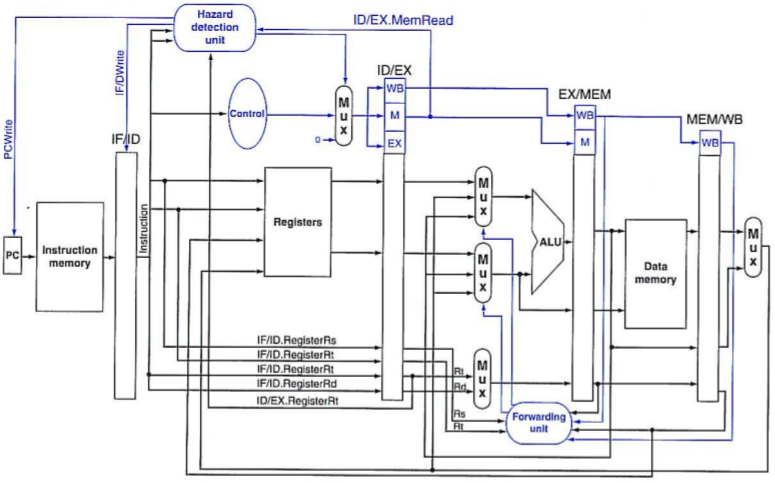
\includegraphics[width=1\textwidth]{figures/mips-pipeline}
        \caption{MIPS pipeline architecture, with hazard detection and data forwarding}
    \label{mips-architecture}
\end{figure}

\subsection{Project files}
The project consisted of the following modules from the last assignment

\begin{itemize}
    \item Com.vhd \hfill \\
        \textit{Communication module, used for programming and controlling the FPGA}
    \item memory.vhd \hfill \\
        \textit{Data memory module}
    \item register\_file.vhd \hfill \\
        \textit{Register module}
    \item alu.vhd \hfill \\
        \textit{Arithmetical Logical Unit}
    \item control\_unit.vhd \hfill \\
        \textit{The main control unit}
    \item alu\_control.vhd \hfill \\
        \textit{ALU control unit}
    \item pc\_register.vhd \hfill \\
        \textit{Program Counter module}
    \item processor.vhd \hfill \\
        \textit{The processor, wiring together all the modules}
    \item mips\_constant\_pkg.vhd \hfill \\
        \textit{File that includes constants and signals used by the different components in the exercise}
    \item user\_logic.vhd \hfill \\
        \textit{File connecting the different buses to the different components}
    \item toplevel.vhd \hfill \\
        \textit{File that couples the processor with the user logic}
\end{itemize}
The assignment was to extend the \textit{processor.vhd}-file with a pipeline and
different hazard detection techniques. Most of the
already existing modules were also extended with more logic.
The following files, or modules, were created in this
exercise

\begin{itemize}
    \item if\_id\_reg.vhd \hfill \\
        \textit{The pipeline register between the fetch and decode stages}
    \item id\_ex\_reg.vhd \hfill \\
        \textit{The pipeline register between the decode and execute stages}
    \item ex\_mem\_reg.vhd \hfill \\
        \textit{The pipeline register between the execute and data access stages}
    \item mem\_wb\_reg.vhd \hfill \\
        \textit{The pipeline register between the data access and the write back stages}
    \item pipeline\_constants.vhd \hfill \\
        \textit{A that gathers the different constants that is used throughout the pipeline}
    \item hazard\_detection\_unit.vhd \hfill \\
        \textit{Module to handle read after load, and similar data hazards, between the 
        active instructions in the pipeline. This module handles when the processor should
        stall or bubble}
    \item forwarding\_unit.vhd \hfill \\
        \textit{Module that handles data forwarding in the memory and
        write back stages}
\end{itemize}
We have also implemented test benches for the hazard detection unit and the 
forwarding unit. 